\documentclass[11pt]{article}

%%%%%%%%%%%%%%%%%%
% Basic packages %
%%%%%%%%%%%%%%%%%%

\usepackage[T1]{fontenc}
\usepackage[utf8]{inputenc}
\usepackage[british]{babel}
\usepackage[stretch = 25, shrink = 25, tracking=true, letterspace=30]{microtype}

\usepackage{geometry}
 \geometry{
 a4paper,
 %total={150mm,257mm},
 left=25mm,
 right=25mm,
 top=15mm,
 } % Page Layout
\usepackage[dvipsnames]{xcolor} % Colour
\usepackage{amsmath} % Maths

%%%%%%%%%%%%%%%%%%%
% Tables, figures %
%%%%%%%%%%%%%%%%%%%

\usepackage{float}
\usepackage{graphicx} % Imgages, figures
\graphicspath{{./figures/}} % Set figure path

\usepackage{booktabs} % Pretty tables

%%%%%%%%%%%%%
% Citations %
%%%%%%%%%%%%%

\usepackage[
    backend=biber,
    style=apa,
    sortlocale=de_DE,
    natbib=true,
    url=false, 
    doi=true,
    eprint=false
]{biblatex}

%\addbibresource{ASSIGNMENT_1.bib} %Imports bibliography file
\usepackage{csquotes} % used for block quotes

%%%%%%%%%
% Fonts %
%%%%%%%%%

%%% Helvetica:
%\usepackage[scaled=0.95]{helvet} % Imports Helvetica, which is similar to Arial
%\renewcommand{\rmdefault}{phv} % Use Helvetica

%%% Atkinson Hyperlegible, nerdy font 
%\usepackage[sfdefault]{atkinson} %% Option 'sfdefault' if the base
%% font of the document is to be sans serif.
%\usepackage[T1]{fontenc}

%%%%%%%%%%%%%%%%%%
% Header setting %
%%%%%%%%%%%%%%%%%%

\usepackage{titlesec} % pretty headers
\titleformat{\section}
  {\normalfont\large\bfseries\color{Black}} % Formatting options
  {\thesection}{1em}{}

%%%%%%%%%%%%%%%%%%
% Title settings %
%%%%%%%%%%%%%%%%%%

\title{\textcolor{Red}{\textbf{COMP527 - CA Assignment 2 - Clustering}}}
\author{\textbf{Pablo Ramos - 201885602}}

\setlength\parindent{10mm}

%%%%%%%%%%%%
%%% BODY %%%
%%%%%%%%%%%%

\begin{document}
% Dark Mode - Comment the bottom 2 lines to get a normal white page
%\pagecolor{black}
%\color{white} % Set the default colour to white
%
%\pagenumbering{gobble} % Turns off page numbering
%
\maketitle
{\setlength{\parindent}{0mm}{\color{Black} \rule{\linewidth}{0.5mm}}} % Lines with colour options

\section{Overview of the Pipeline}

\texttt{clustering.py} calls the functions from \texttt{preprocessing.py} to call and clean the data and then uses TF-IDF vectorisation on the data to get a mathematical abstraction of the sentences. Latent Semantic Analysis was used to simplify the geometry of the resulting vector set. L2 normalisation was implemented as well.

This final set was then used to get the silhouette analysis.

\section{Term Frequency - Inverse Document Frequency (TF-IDF)}

TF-IDF is a statistical method that determines the relevance of a word in relation to the document it appears in. In this case, the term frequency for a single term t of a sentence s is described as:

\begin{center}
  $TF=\frac{\text{Frequency of }t}{\text{Count of unique terms in }s}$
\end{center}

{\setlength{\parindent}{0mm}The inverse document frequency is described mathematically as:}

\begin{center}
  $IDF=\log\left(\frac{\text{Total number of sentences}}{\text{Count of sentences with term }t}\right)$
\end{center}

{\setlength{\parindent}{0mm}The final TF-IDF score for a term is the product of both values. Words that appear frequently in a sentence but rarely across the dataset score highly, making them strong signals for distinguishing clusters.}

\section{Latent Semantic Analysis (LSA)}

TF-IDF produces a high-dimensional sparse matrix, which is problematic for clustering due to the curse of dimensionality --- in high-dimensional spaces, distances between points tend to converge, making it harder to form well-separated clusters. LSA addresses this by applying Truncated Singular Value Decomposition (SVD) to reduce the matrix to a lower-dimensional dense representation, whilst preserving the most meaningful semantic relationships between terms.

After experimenting with several values, \texttt{n\_components=10} was selected. Whilst this retains only 6.89\% of the explained variance, it produced the highest silhouette scores and, upon inspection, yielded semantically coherent clusters.

\section{L2 Normalisation}

L2 normalisation was applied to the LSA-reduced matrix, scaling each sentence vector to unit length. This ensures that K-Means computes distances based on the direction of vectors rather than their magnitude, preventing longer sentences from dominating the clustering simply due to having more terms.

\section{Silhouette Analysis}

Silhouette analysis was used to determine the optimal number of clusters $K$. For each data point, the silhouette coefficient $s$ is defined as:

\begin{center}
  $s = \frac{b - a}{\max(a, b)}$
\end{center}

{\setlength{\parindent}{0mm}where $a$ is the mean intra-cluster distance and $b$ is the mean distance to the nearest neighbouring cluster. The overall score for a given $K$ is the average across all points, with values ranging from $-1$ (poor) to $1$ (ideal). K-Means was run for $K = 1$ to $10$, with $K=1$ hardcoded to a score of 0 as the coefficient is undefined for a single cluster.}

\begin{figure}[h]
  \centering
  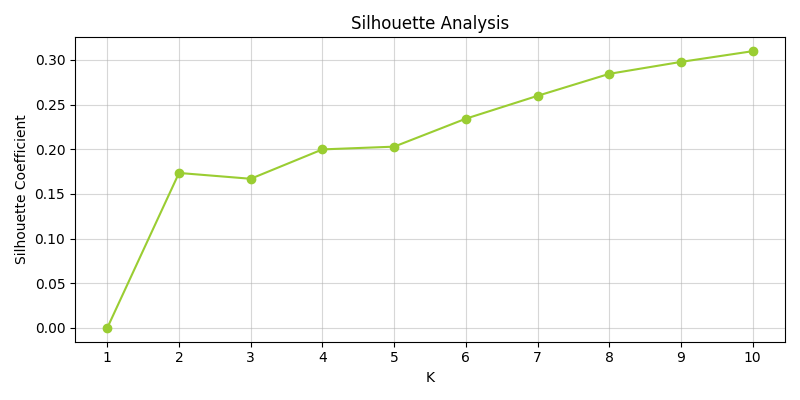
\includegraphics[width=0.8\textwidth]{las_silhouette_plot_tuned.png}
  \caption{Silhouette coefficients for $K = 1$ to $10$.}
  \label{fig:silhouette}
\end{figure}

\section{Optimal $K$ and Results}

As shown in Figure \ref{fig:silhouette}, silhouette scores increase consistently with $K$, peaking at $K=10$ with a score of 0.3097. This was selected as the optimal value. Inspection of the resulting clusters revealed genuine semantic structure --- Shakespeare dialogue was sub-clustered by character and scene, whilst reviews were grouped broadly by length and style. The relatively low absolute scores reflect the mixed nature of the dataset rather than a failure of the method.

%\begin{displayquote}
%    This is some text from a book.
%\end{displayquote}

%%%%%%%%%%%%%%%%%%%%%%
% Implicit citations %
%%%%%%%%%%%%%%%%%%%%%%

%\nocite{Hunter:2007}
% \nocite{Waskom2021}


 %\printbibliography

\end{document}